\documentclass{article}
\usepackage{gensymb, amsmath, float, graphicx, epstopdf}
\restylefloat{table}
\usepackage[margin=0.75in]{geometry}
\begin{document}

\title{Lab 2: The Smith Chart Data}
\author{Michael Shen}
\date{}
\maketitle


\section{Line Parameters of a Lossless Line}

\subsection{Measured Data}

\begin{table}[h]
\centering
	\begin{tabular}{rl}
	Patch Cord Length =  	  & 0.6229 $m$  \\
	Added Electrical Delay =  & 6.2565 $ns$
	\end{tabular}
\end{table}

\section{Lossy and Lossless Lines on the Smith Chart}
\subsection{Measured Data}
No Data.


\section{Impedance Measurements Using the Smith Chart}

\subsection{Measured Data}
\begin{table}[H]
\centering
	\begin{tabular}{rl}
	Resistor =   & 10 $\Omega$  \\
	Capacitor =  & 39 $pF$
	\end{tabular}
\end{table}

\begin{table}[H]
\centering
\begin{tabular}{|l|l|l|l|l|}
\hline
\multicolumn{1}{|c|}{\textbf{Load}} & \multicolumn{1}{c|}{\textbf{400 MHz}} & \multicolumn{1}{c|}{\textbf{600 MHz}} & \multicolumn{1}{c|}{\textbf{800 MHz}} & \multicolumn{1}{c|}{\textbf{1.0 GHz}} \\ \hline
Short                               & 0.06031 + j2.208                      & 0.07049 + j3.2748                     & 0.1680 + j4.621                       & 0.01835 + j5.789                      \\ \hline
Open                                & 51.12 - j927.1                        & -16.49 - j713.9                       & -3.485 - j483.5                       & 8.908 - j304.2                        \\ \hline
Resistive                           & 11.57 + j19.34                        & 14.05 + j31.05                        & 18.65 + j45.98                        & 28.90 + j66.99                        \\ \hline
Capacitive                          & 2.895 - j750.6                        & 1.832 - j524.7                        & -2.166 - j377.4                       & 10.91 - j293.2                        \\ \hline
Series                              & 11.10 + j11.26                        & 14.76 + j28.21                        & 23.72 + j50.55                        & 52.46 + j88.62                        \\ \hline
Parallel                            & 5.481 + j12.63                        & 2.812 + j23.19                        & 1.168 + j35.15                        & 341.0 + j48.125
\\ \hline
\end{tabular}
	\caption{Voltage and phase measurements for varying signal frequency and cable length}
	\label{Data 1}
\end{table}

\section{Impedance Matching Using a Single Stub Tuner}

\subsection{Measured Data}

\begin{table}[H]
\centering
	\begin{tabular}{rl}
	Impedance before Matching =   			 & 23.79 + j63.00 $\Omega$  \\
	Distance between Load and Stub Tuner =   & 2.54 $cm$  \\
	Length of Stub =   						 & 11.2713 $cm$  \\
	Impedance after Matching =  			 & 185.5 - j11.54 $\Omega$
	\end{tabular}
\end{table}

\section{Figures and Images}
\begin{figure}[H]
    \centering
    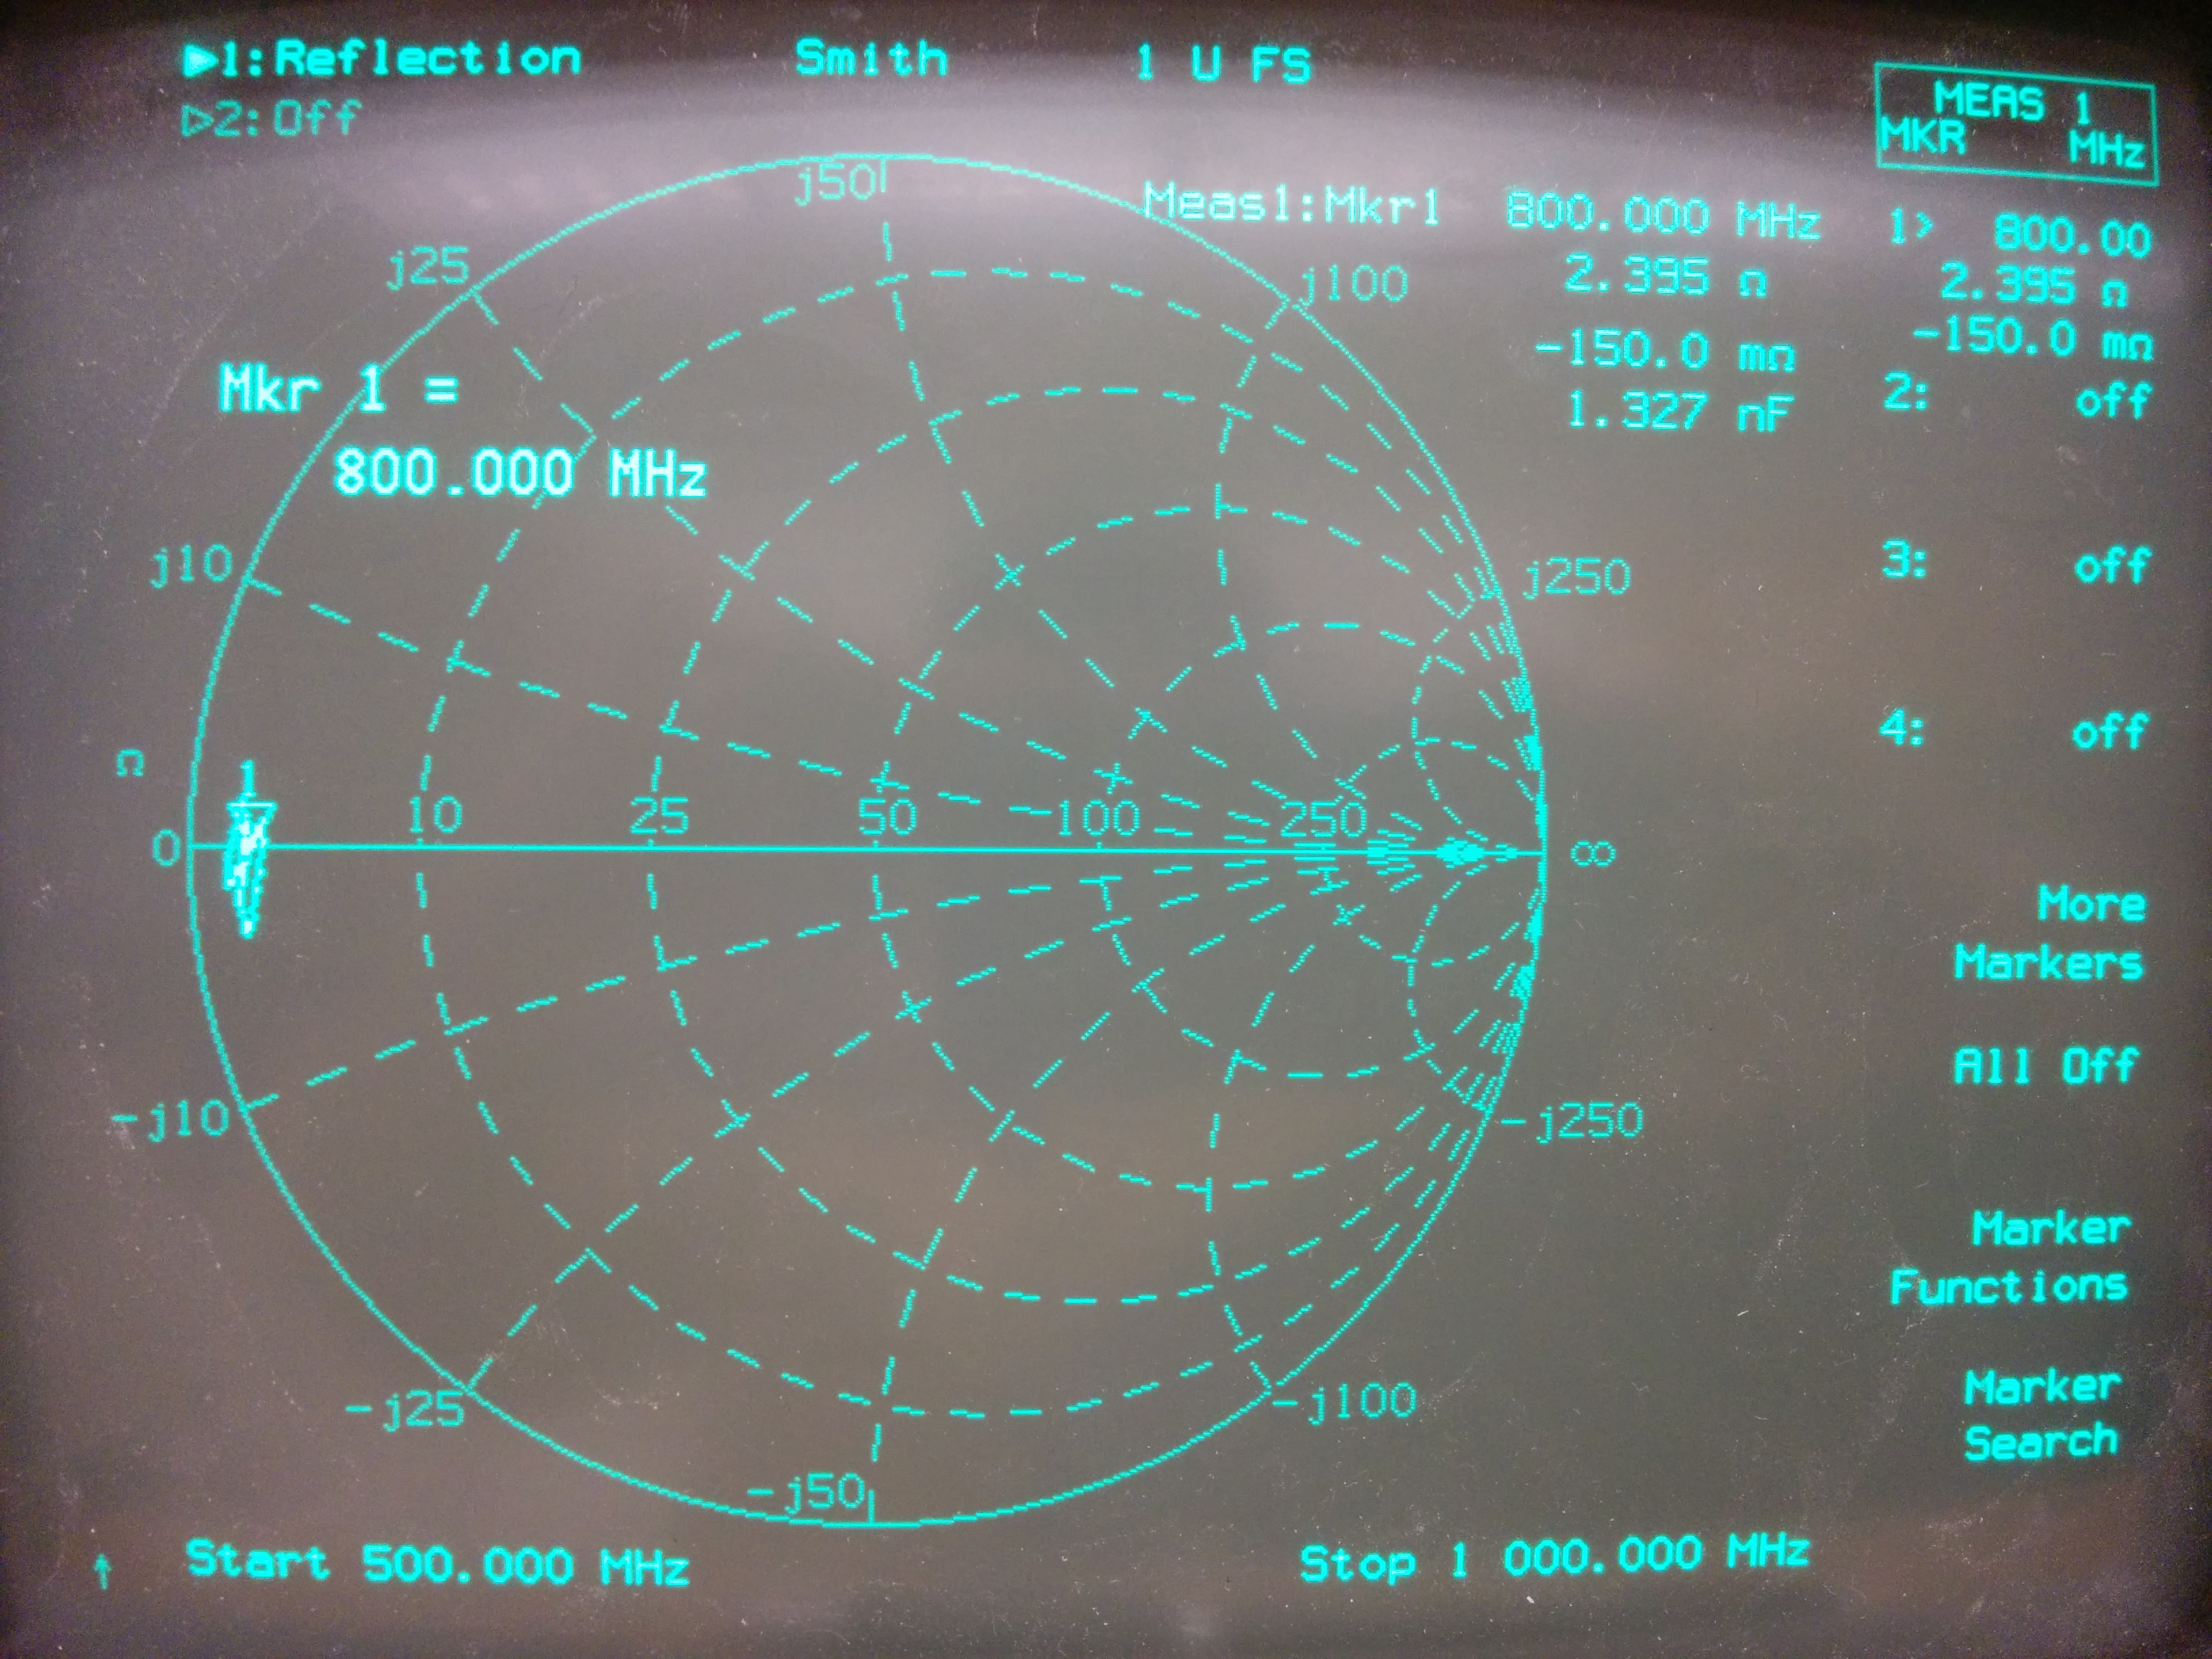
\includegraphics[width=0.8\textwidth]{./Images/251.jpg}
    \caption{Point-like response for a lossless line}
\end{figure}
\begin{figure}[H]
    \centering
    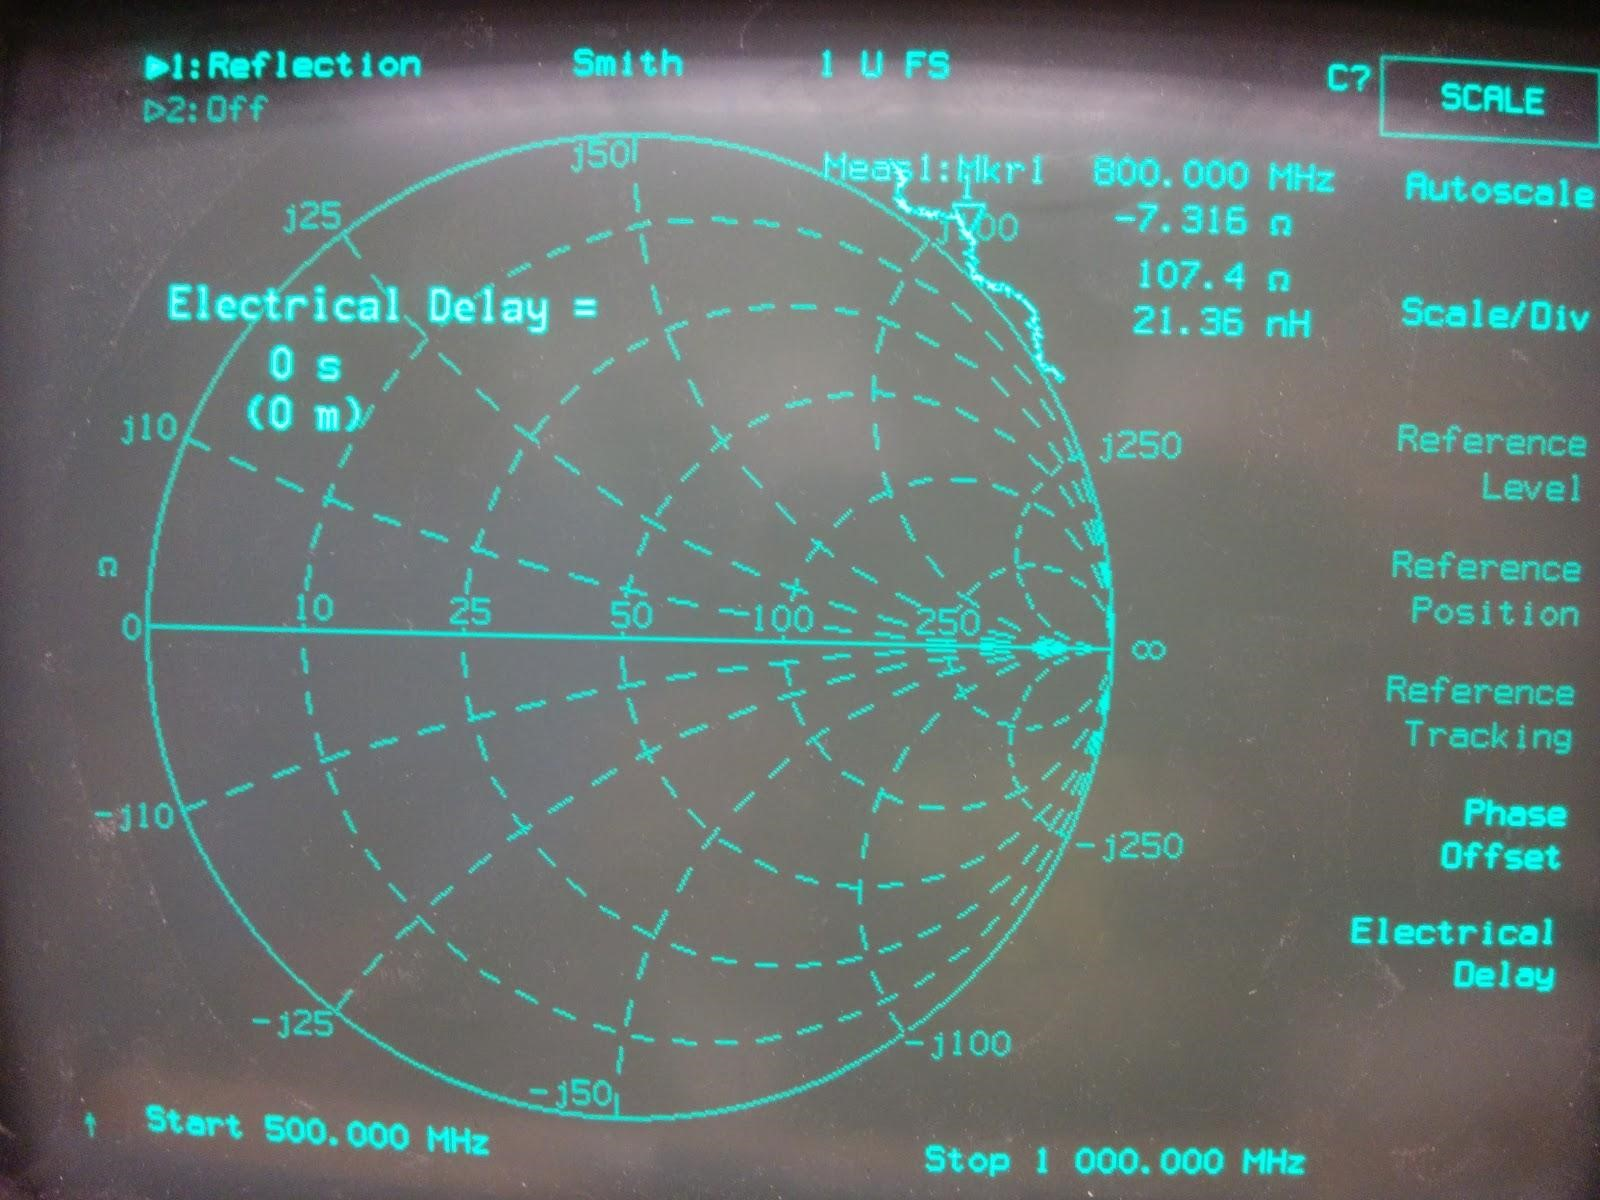
\includegraphics[width=0.8\textwidth]{./Images/252lossless.jpg}
    \caption{Network Analyzer response for a lossless line}
\end{figure}
\begin{figure}[H]
    \centering
    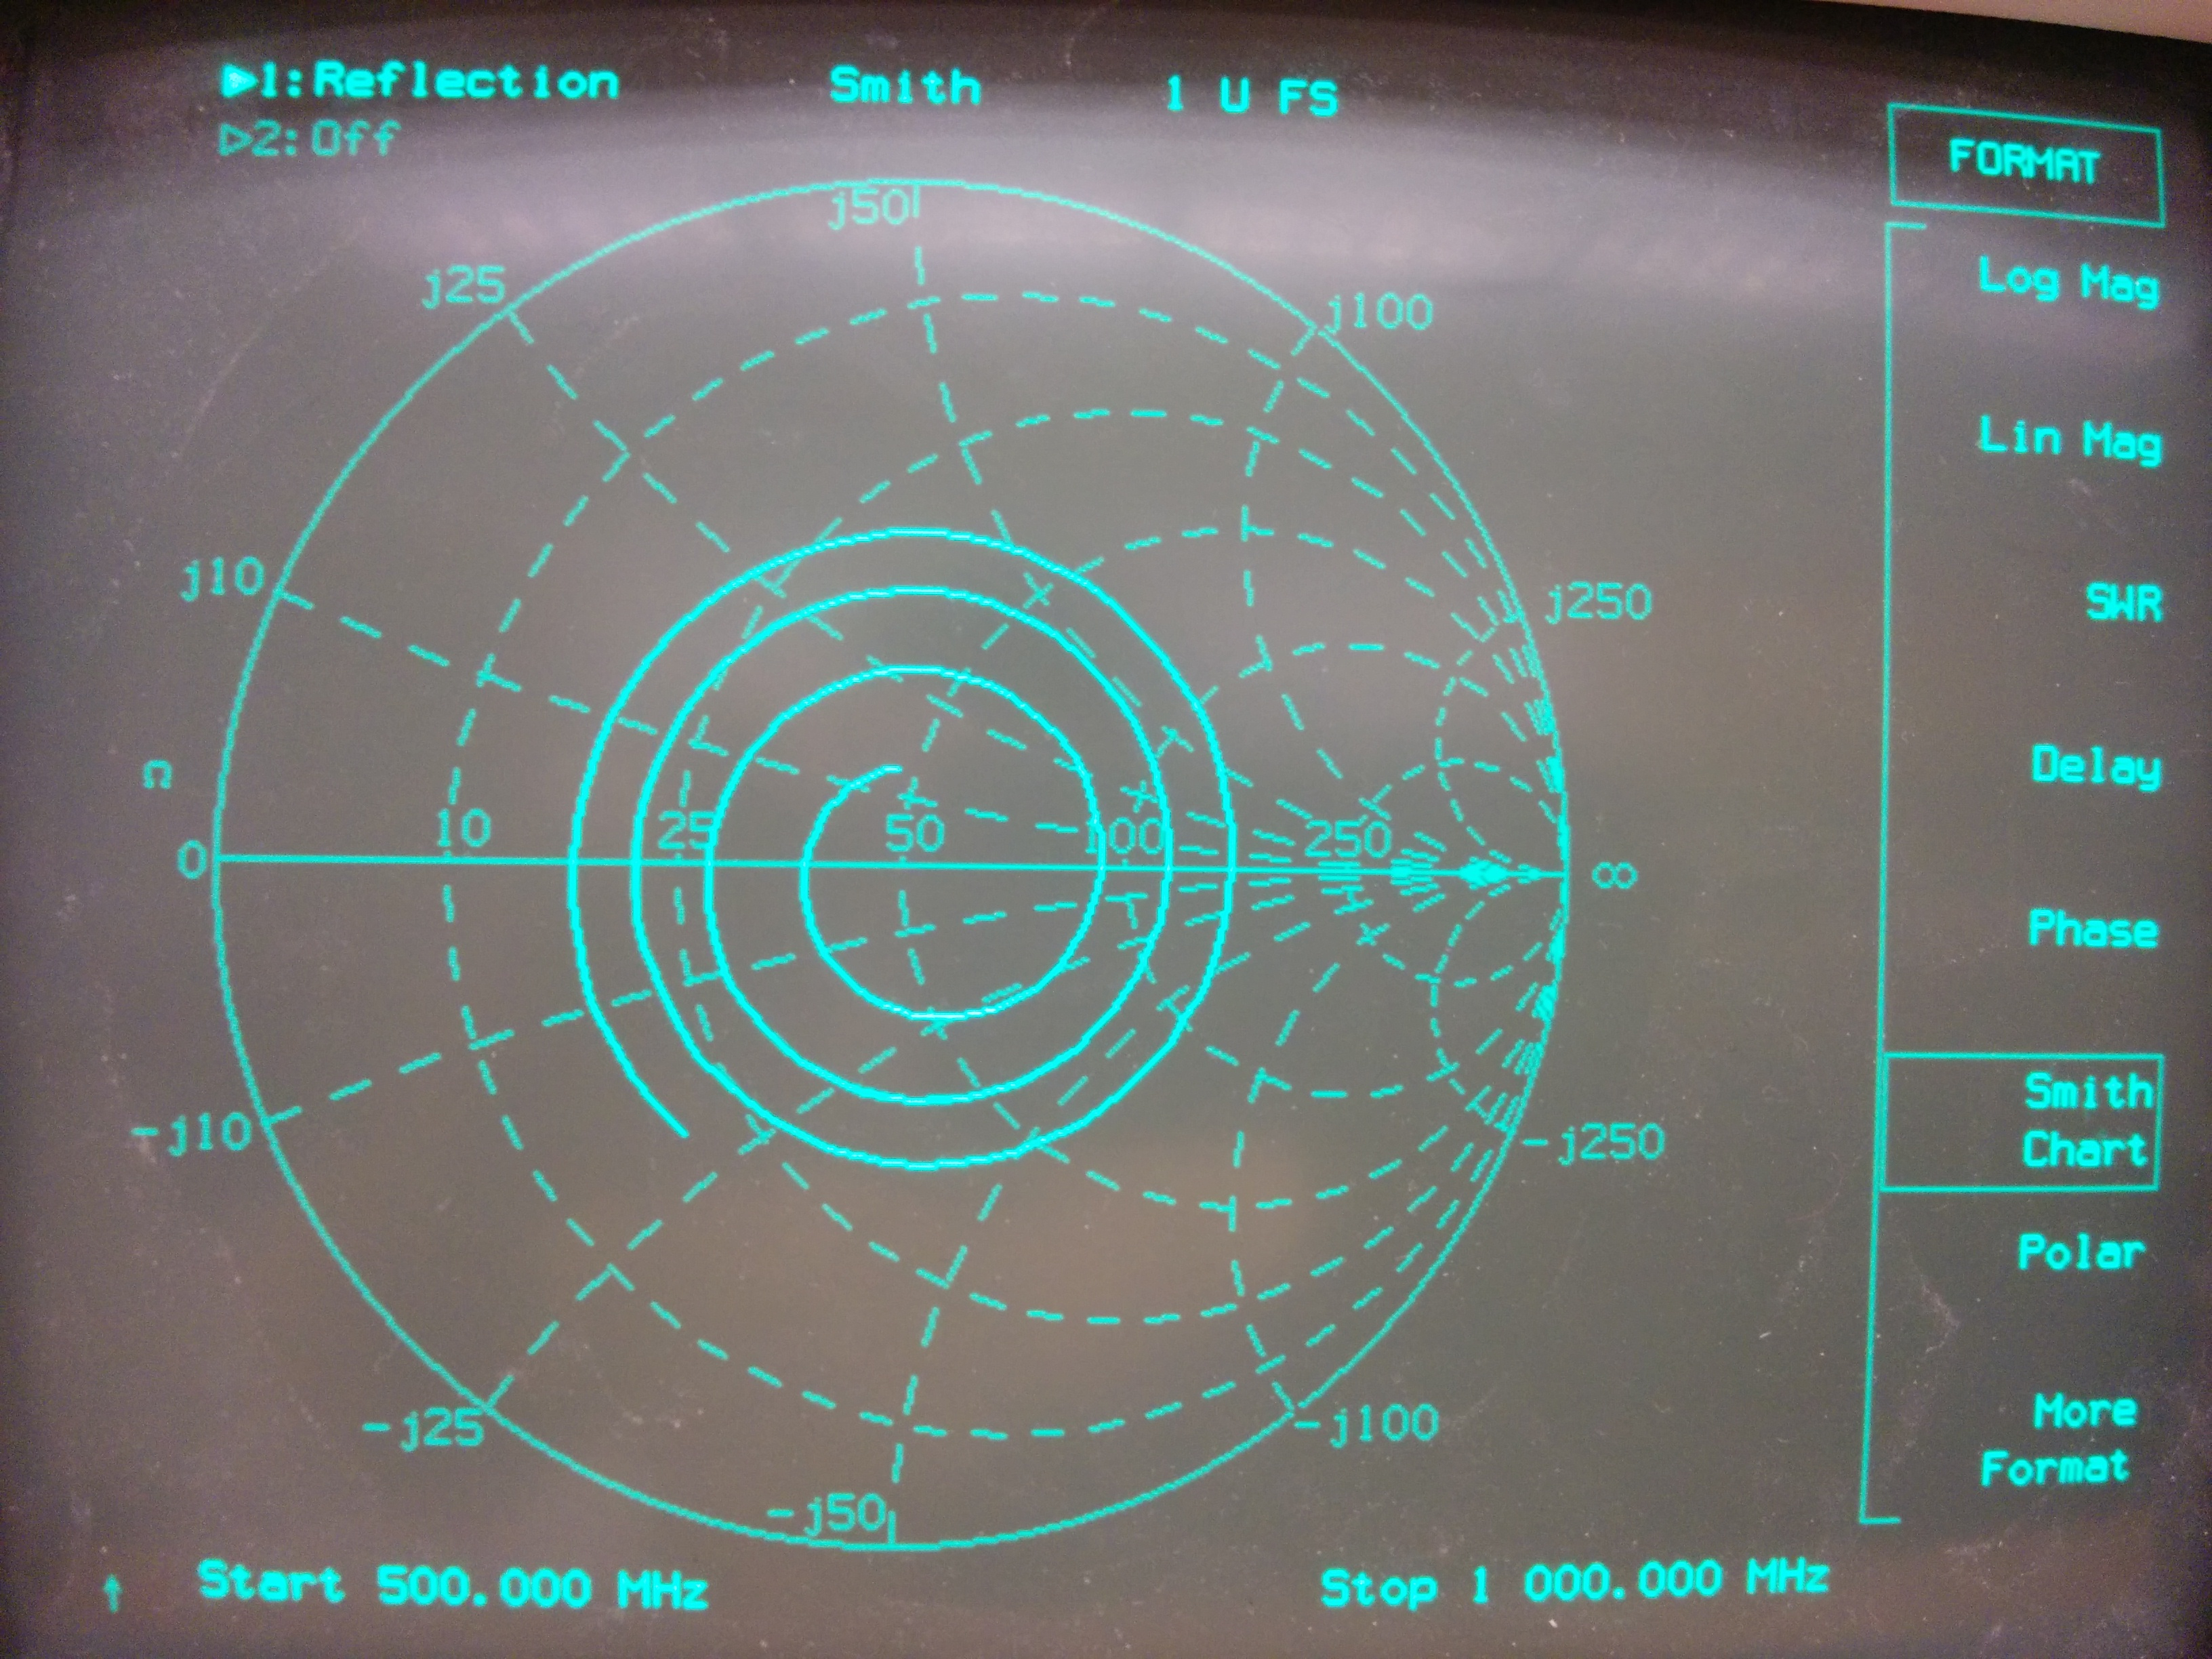
\includegraphics[width=0.8\textwidth]{./Images/252lossy.jpg}
    \caption{Network Analyzer response for a lossy line}
\end{figure}
\begin{figure}[H]
    \centering
    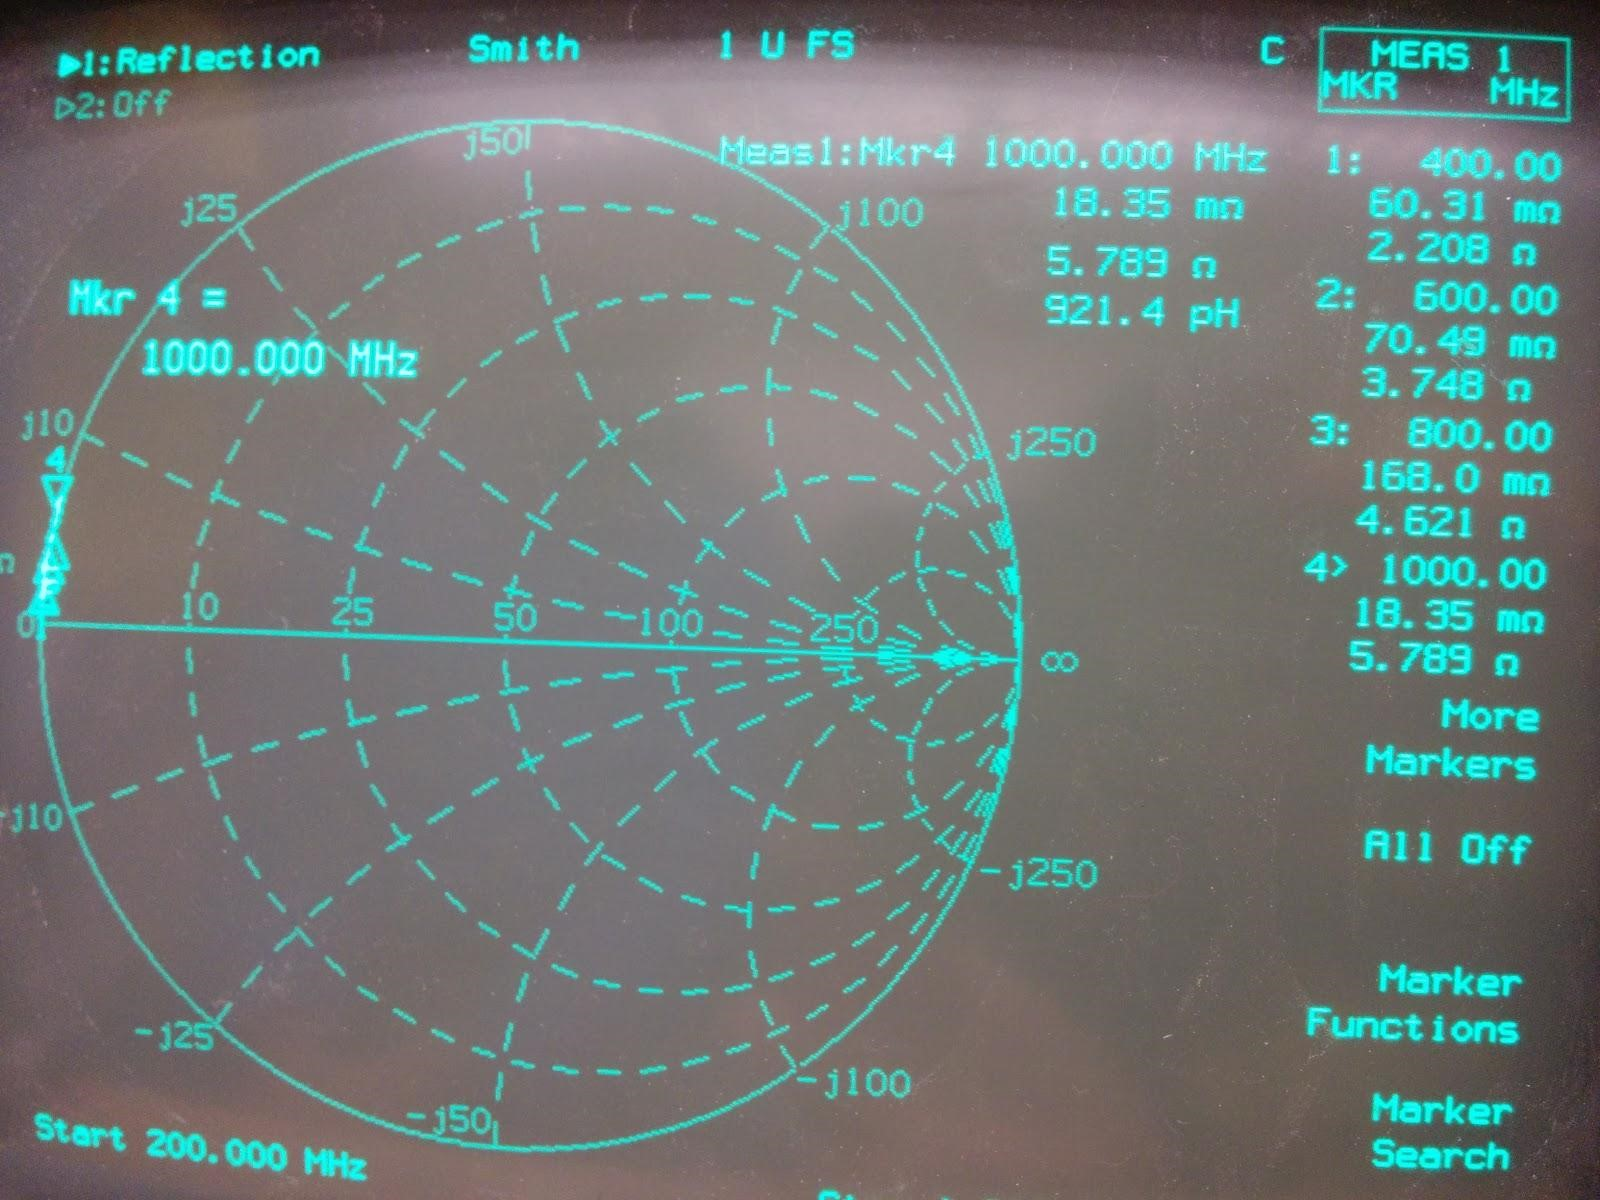
\includegraphics[width=0.8\textwidth]{./Images/253short.jpg}
    \caption{Network Analyzer response for a shorted load}
\end{figure}
\begin{figure}[H]
    \centering
    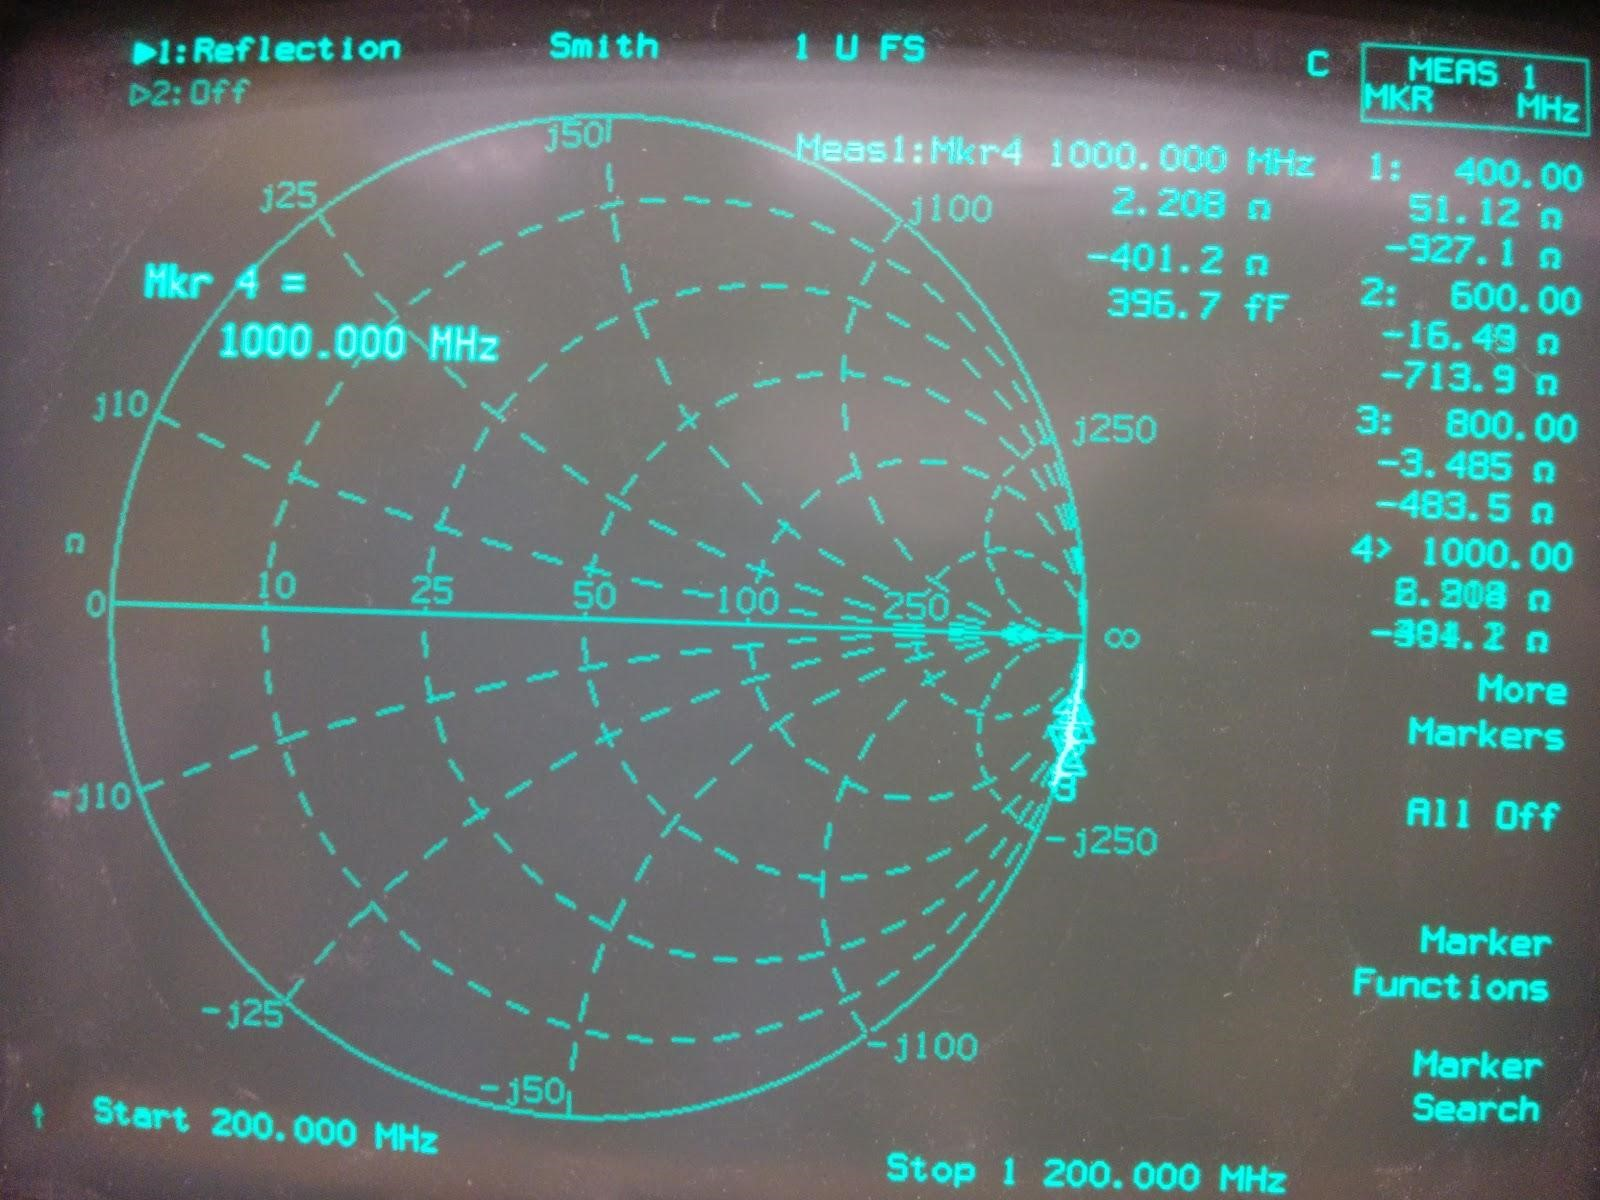
\includegraphics[width=0.8\textwidth]{./Images/253open.jpg}
    \caption{Network Analyzer response for an open load}
\end{figure}
\begin{figure}[H]
    \centering
    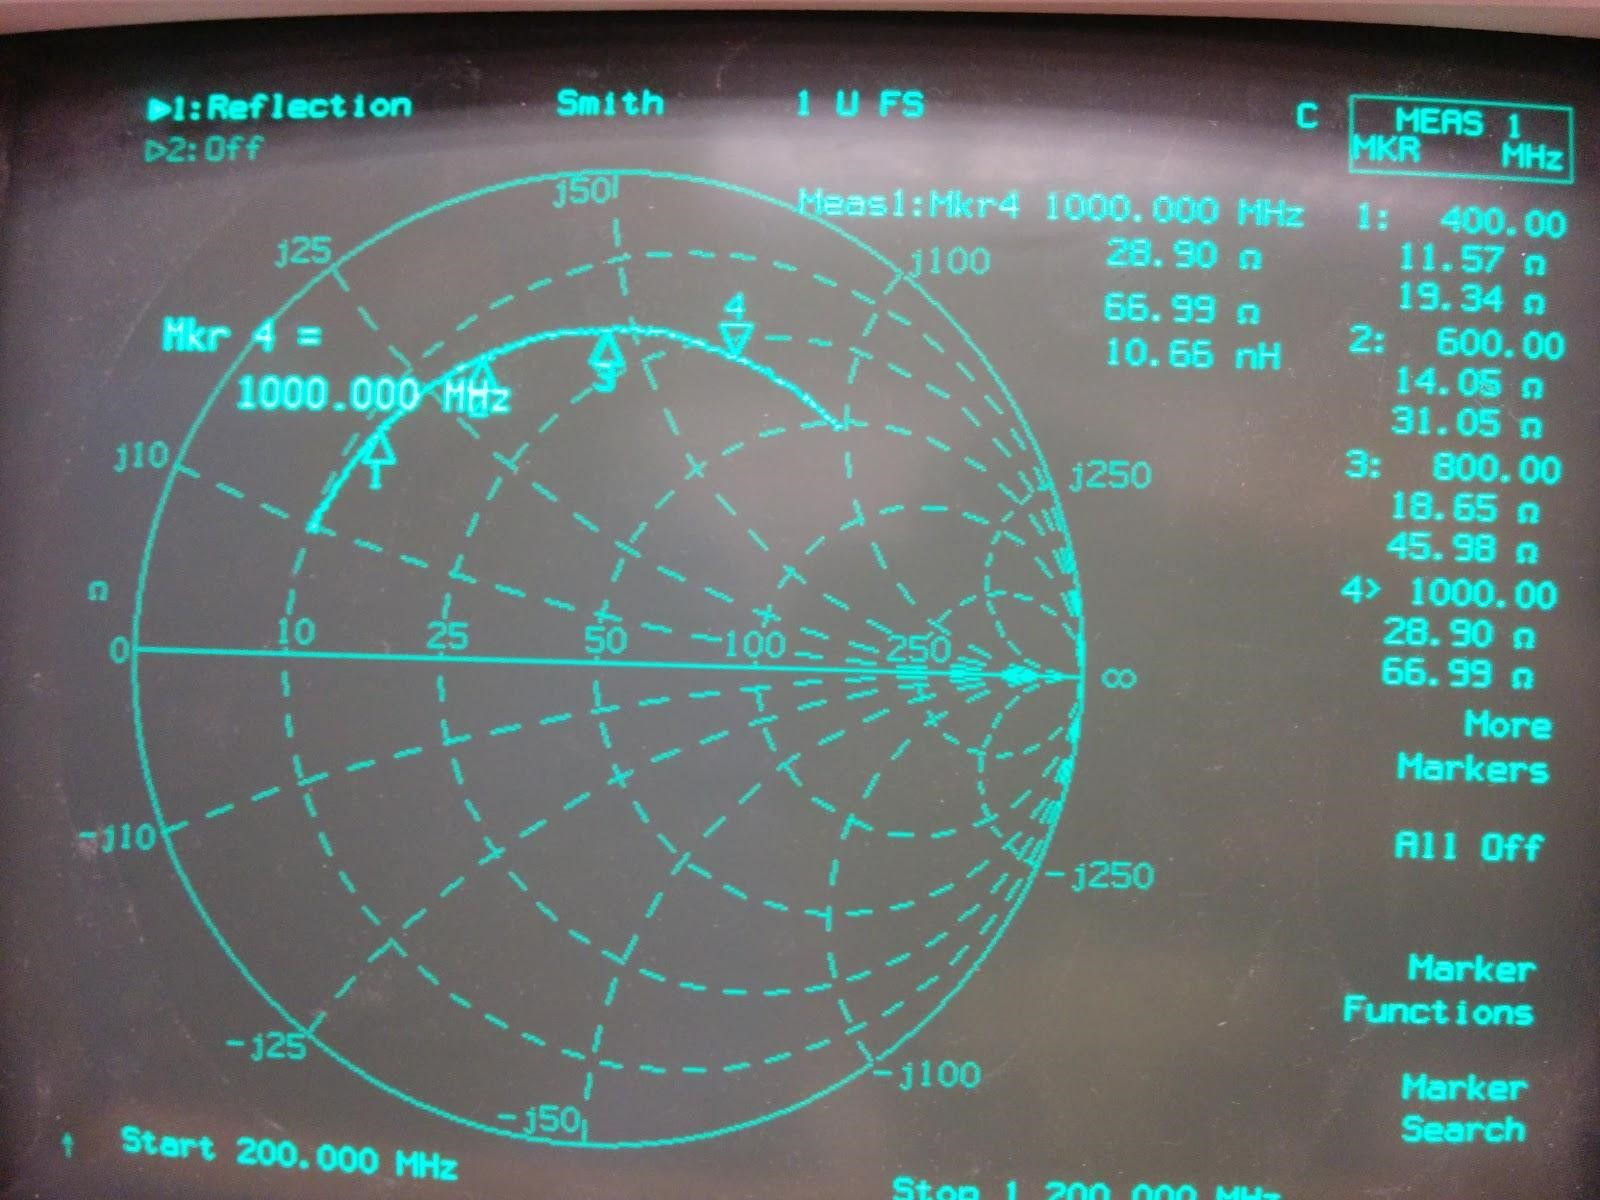
\includegraphics[width=0.8\textwidth]{./Images/253resisitive.jpg}
    \caption{Network Analyzer response for a resistive load}
\end{figure}
\begin{figure}[H]
    \centering
    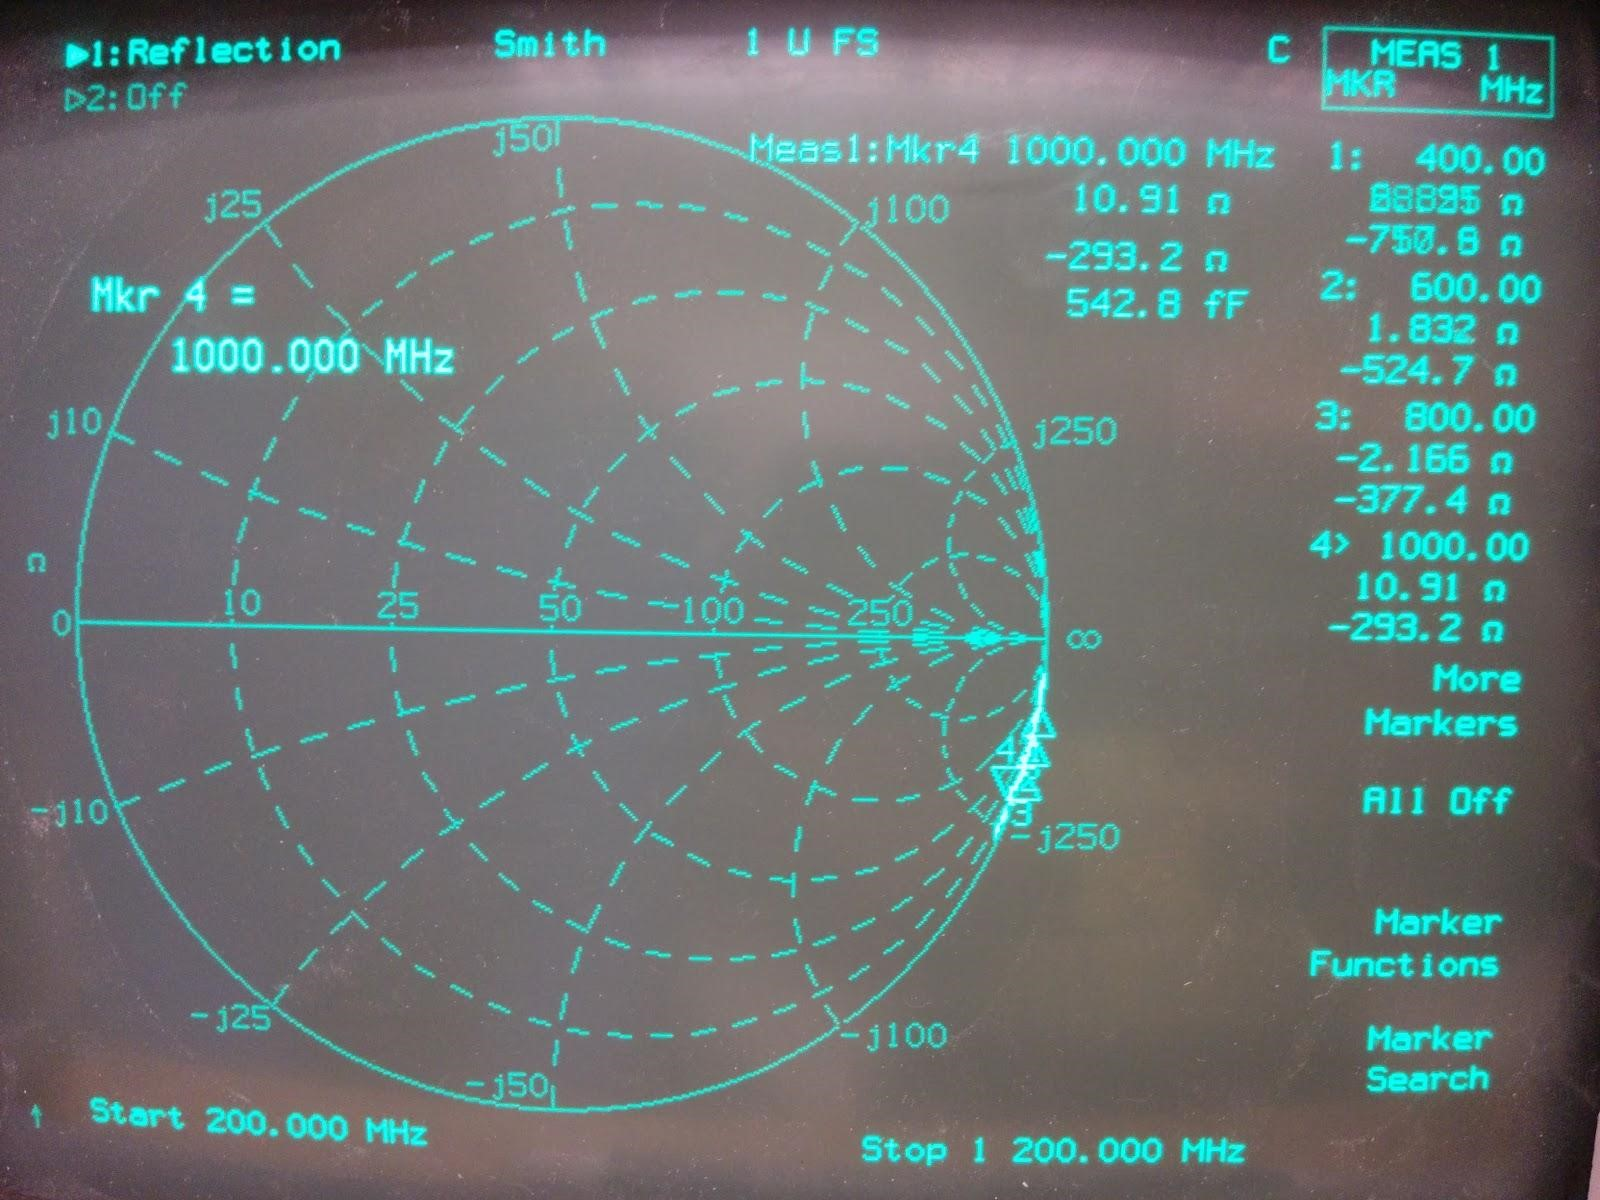
\includegraphics[width=0.8\textwidth]{./Images/253capacitive.jpg}
    \caption{Network Analyzer response for a capacitive load}
\end{figure}
\begin{figure}[H]
    \centering
    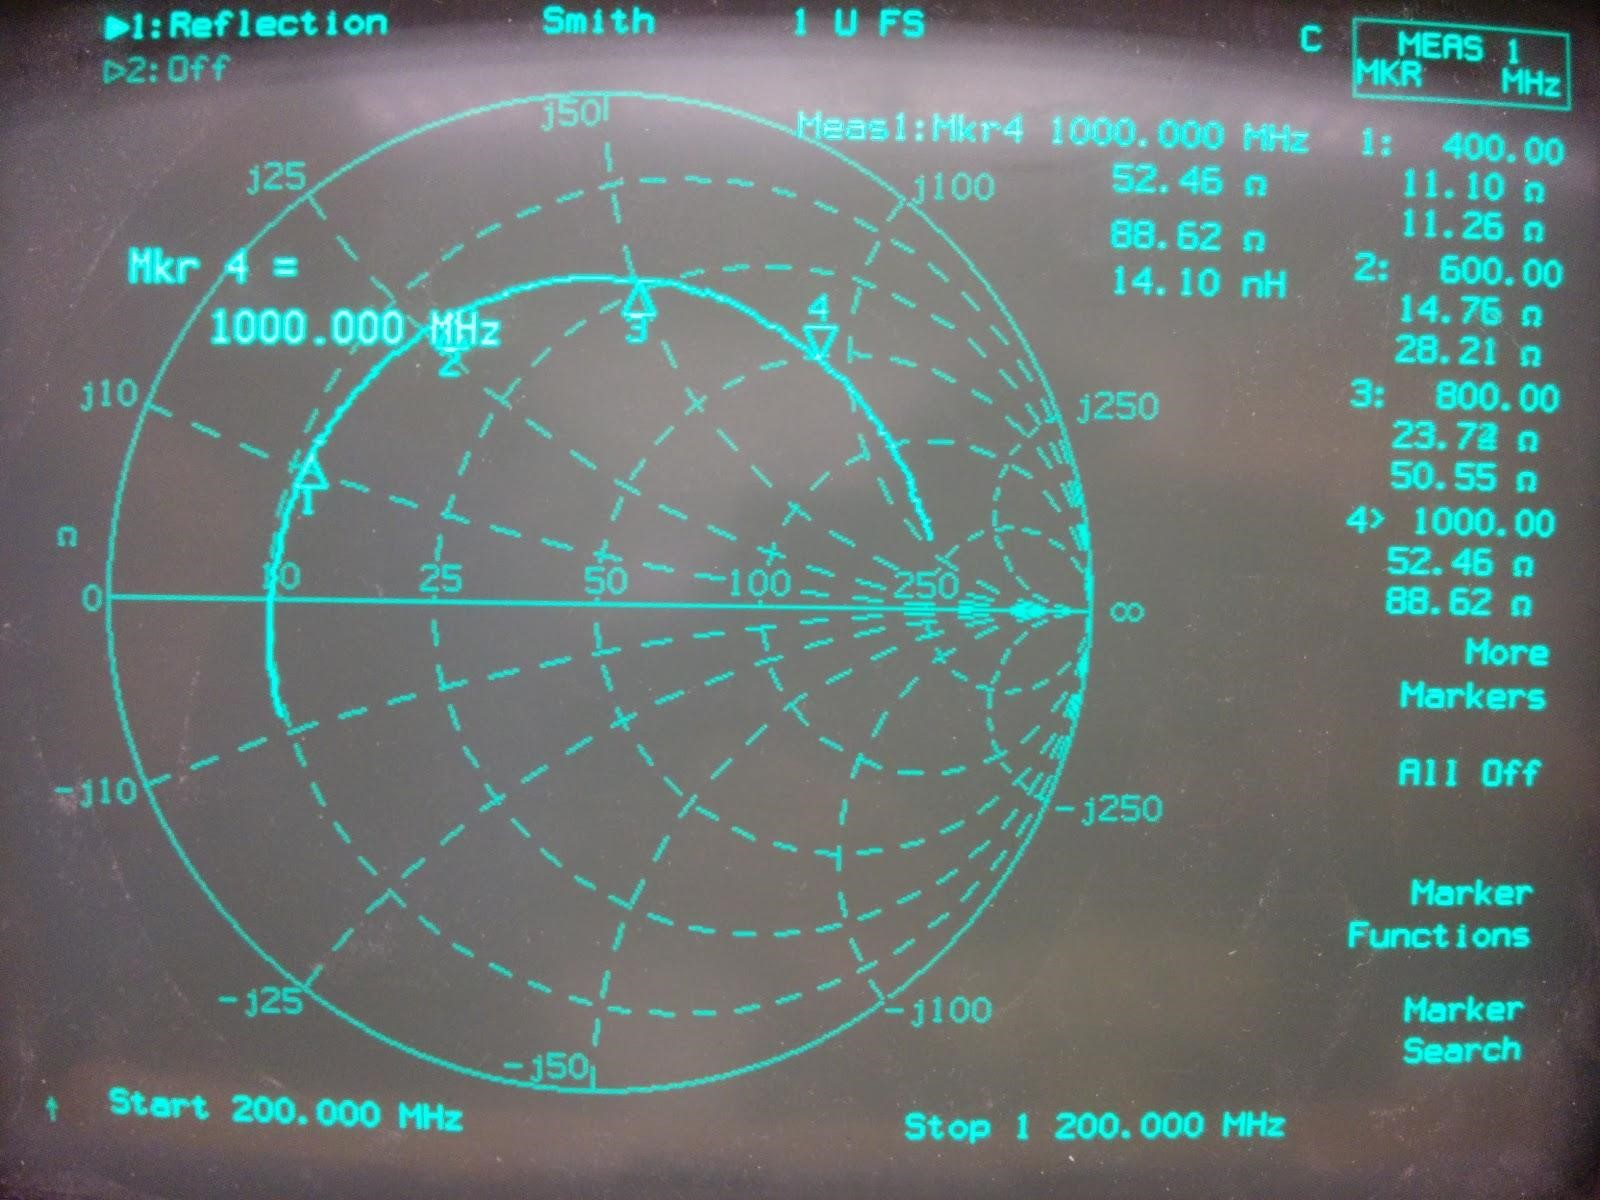
\includegraphics[width=0.8\textwidth]{./Images/253series.jpg}
    \caption{Network Analyzer response for a series load}
\end{figure}
\begin{figure}[H]
    \centering
    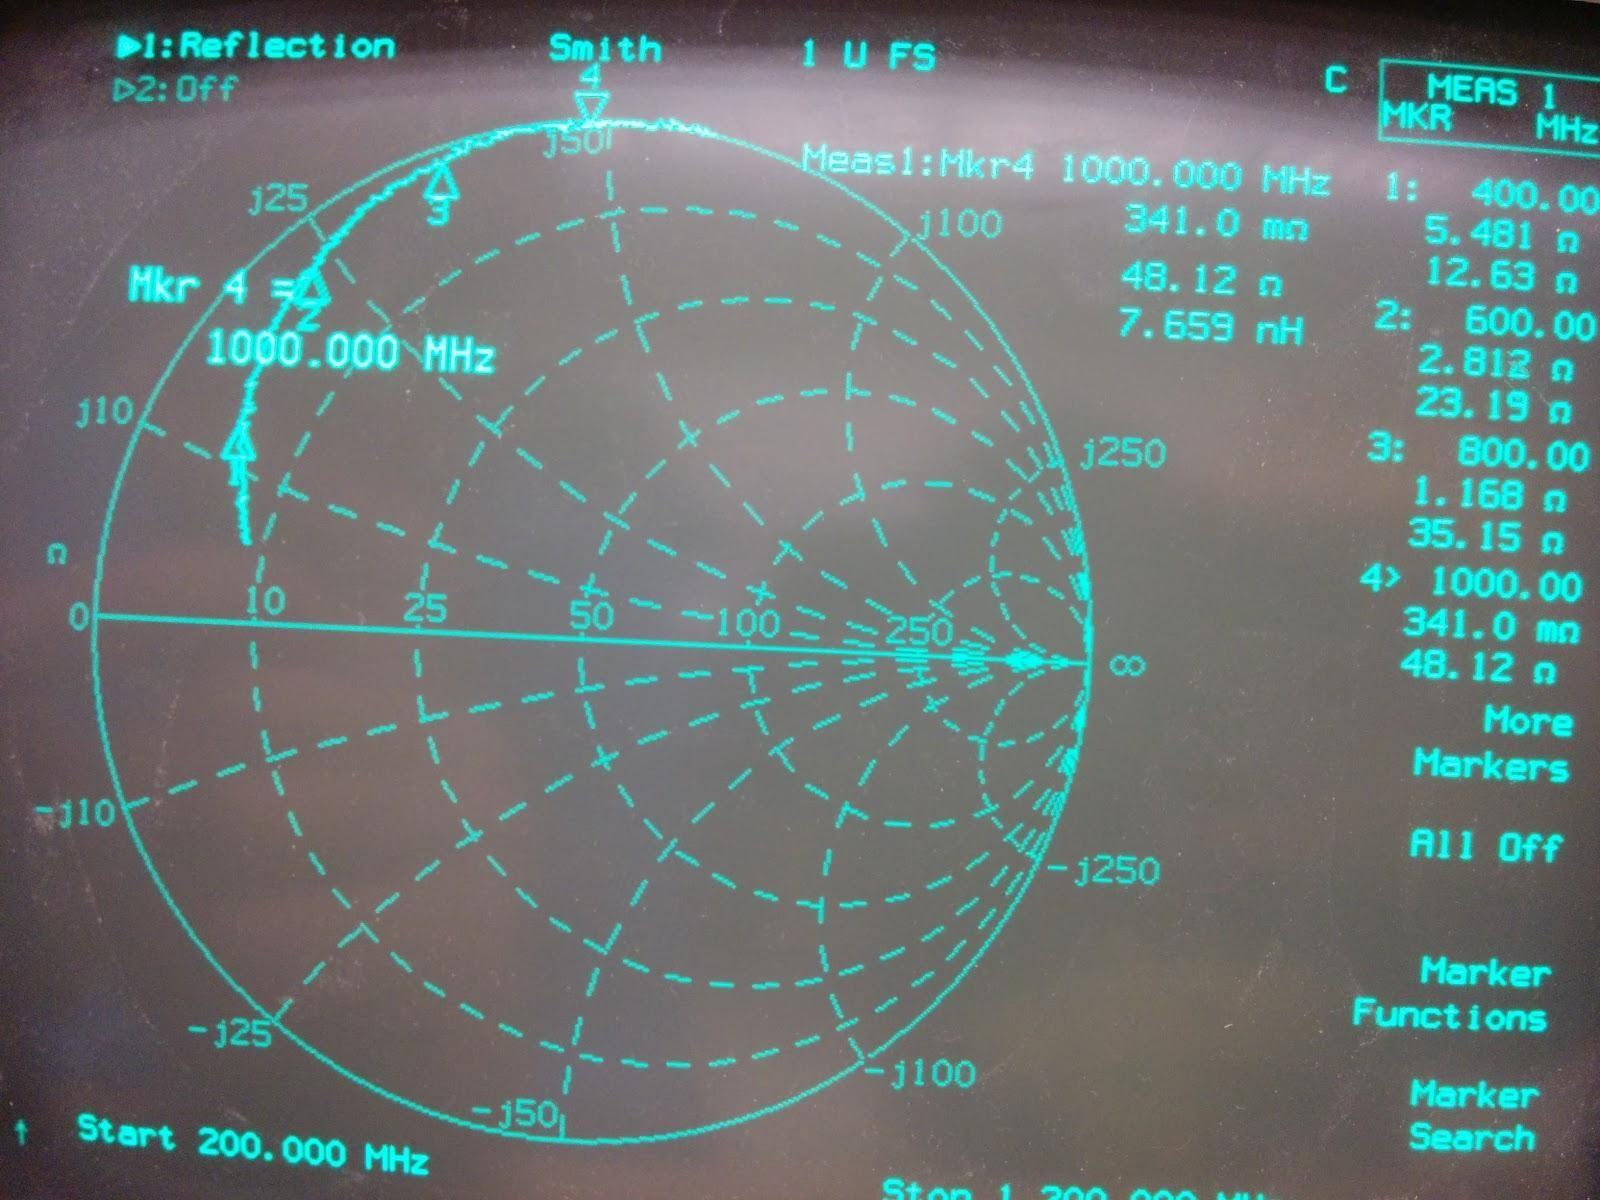
\includegraphics[width=0.8\textwidth]{./Images/253parallel.jpg}
    \caption{Network Analyzer response for a parallel load}
\end{figure}
\begin{figure}[H]
    \centering
    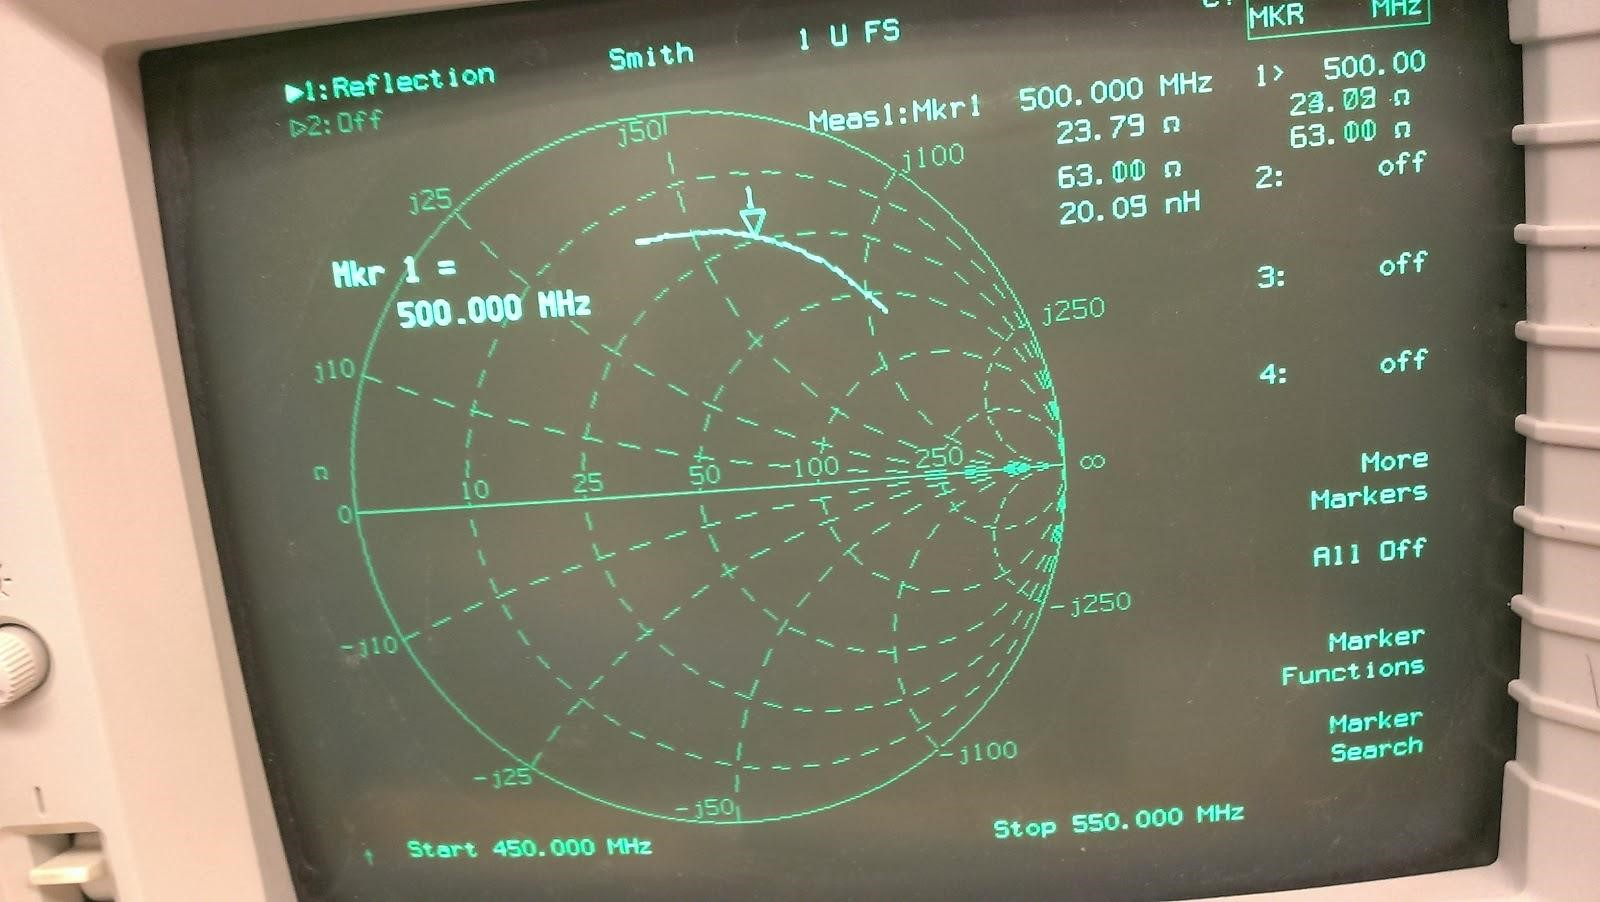
\includegraphics[width=0.8\textwidth]{./Images/254noadj.jpg}
    \caption{Network Analyzer response for the unmatched load}
\end{figure}
\begin{figure}[H]
    \centering
    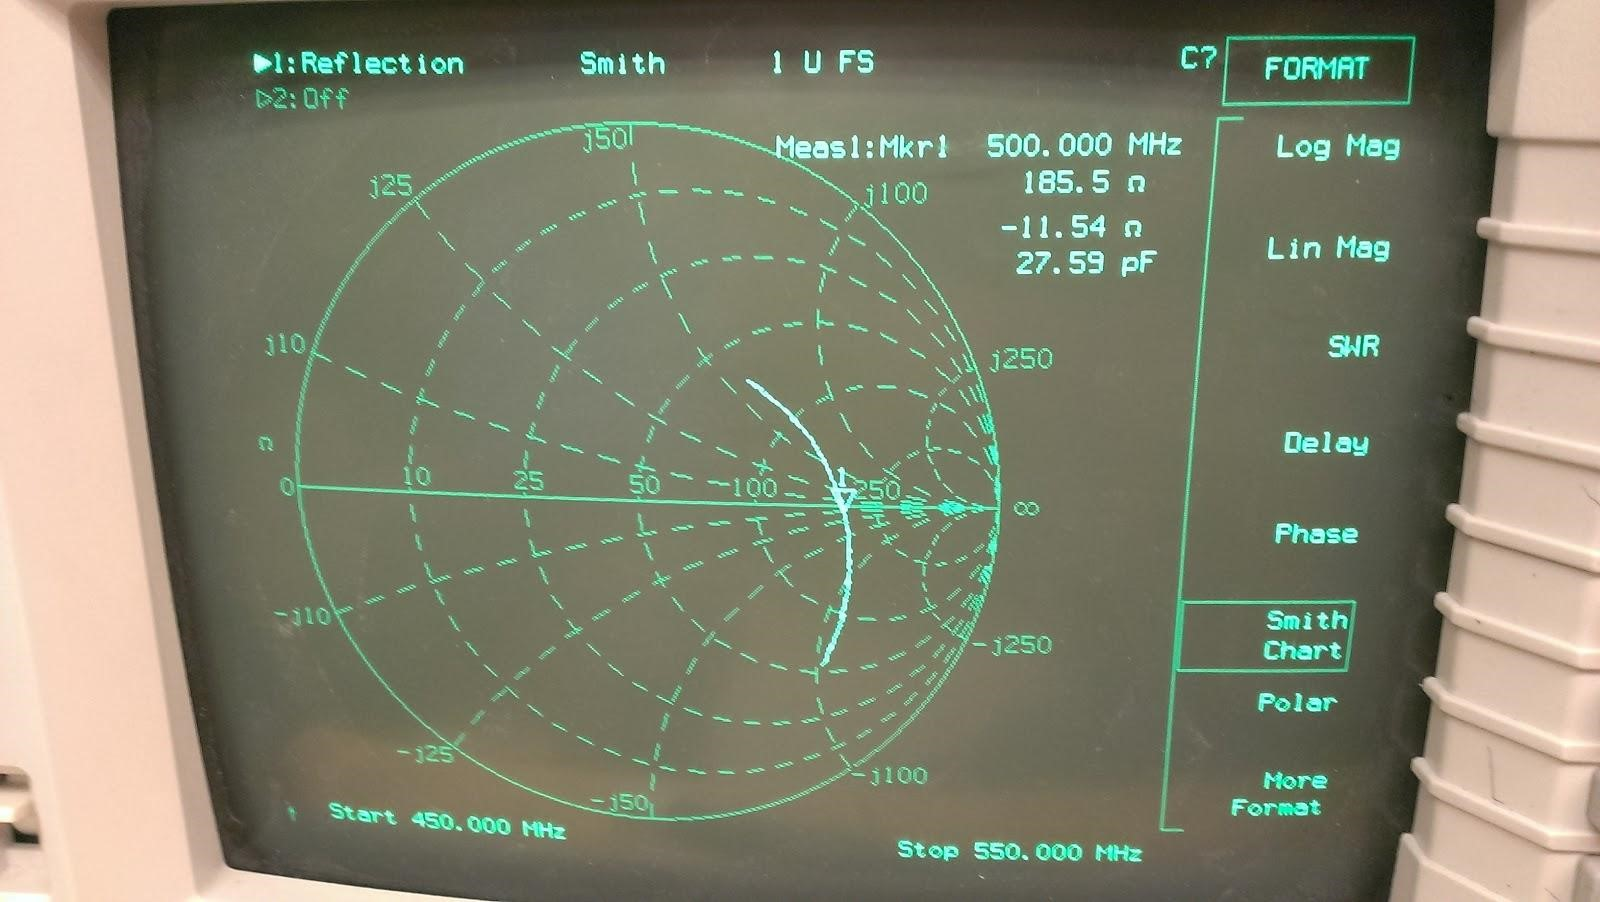
\includegraphics[width=0.8\textwidth]{./Images/254adj.jpg}
    \caption{Network Analyzer response for the matched load with the shorted stub}
\end{figure}
\end{document}